\section{WhatsApp Integration Layer}
\label{sec:whatsapp_integration}

Integrating with WhatsApp presents a significant constraint: the platform's End-to-End Encryption (E2EE) implementation, based on the Signal protocol, means that message content is inaccessible to any external intermediary. To process incoming messages for task extraction, Chatnalyxer deploys the \texttt{Baileys} Node.js library as a headless edge client. The system operates through a user-authorized WhatsApp Web session established on the user's own device. Messages are processed only after successful authentication initiated by the user. Rather than routing through third-party servers, \texttt{Baileys} performs the Signal protocol handshake directly on the local machine, exposing decrypted message events as a local Node.js event stream (illustrated in Fig.~\ref{fig:uml_sequence}).

\begin{figure}[tbp]
    \centering
    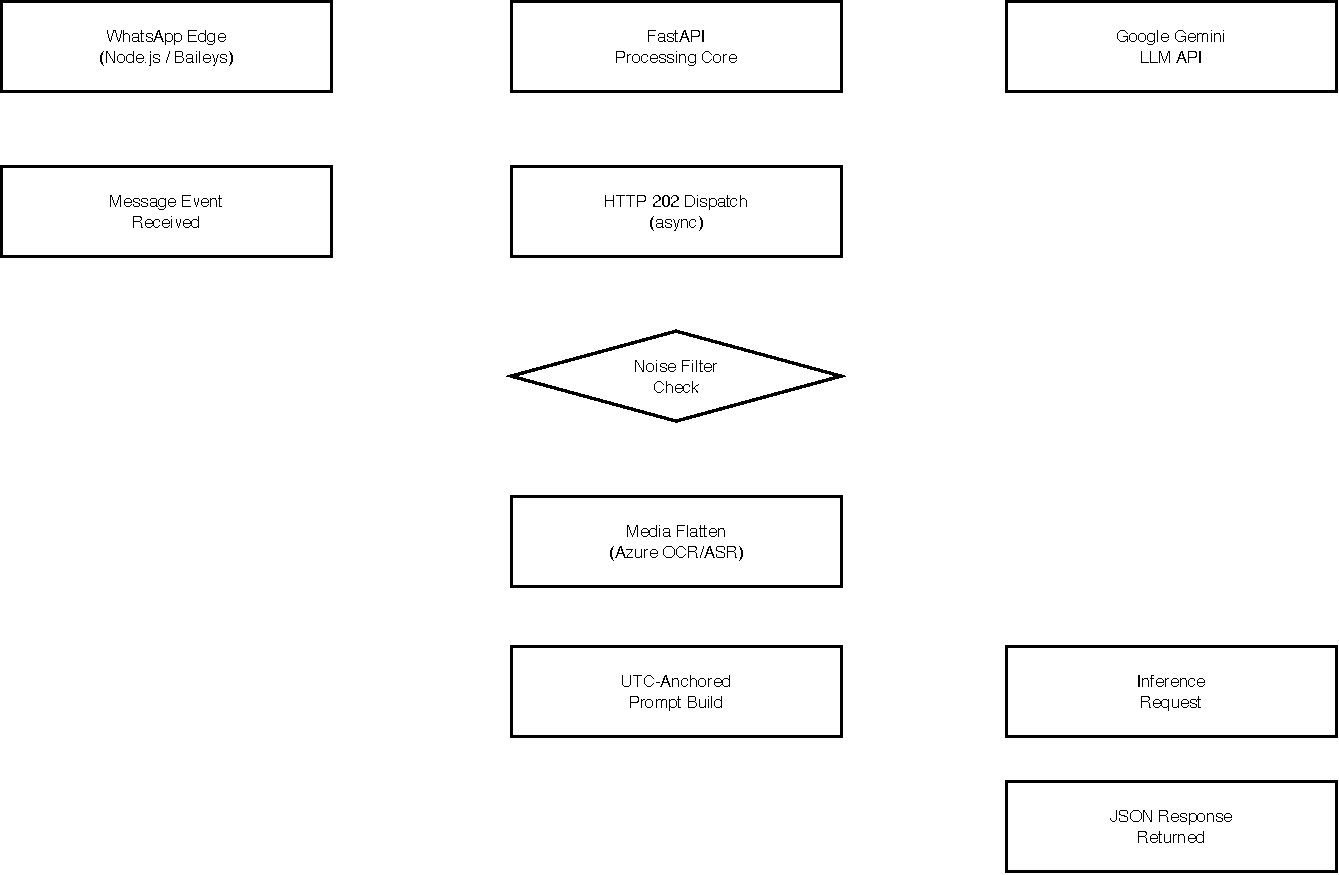
\includegraphics[width=0.95\columnwidth,keepaspectratio]{figures/Fig4_Sequence_Diagram.pdf}
    \setlength{\abovecaptionskip}{4pt}
    \setlength{\belowcaptionskip}{-4pt}
    \caption{UML Sequence Diagram illustrating the E2EE WebHook edge dispatch flow. The edge client filters status updates, reactions, and other non-actionable events before forwarding substantive message payloads to the FastAPI core.}
    \label{fig:uml_sequence}
\end{figure}

Not every event emitted by the WhatsApp protocol represents a user-authored message. Status updates, read receipts, and message reactions are high-frequency events with zero task-extraction value. Passing them to the inference layer would introduce unnecessary latency and API cost. As formalized in Algorithm~\ref{alg:message_filtration}, the integration layer applies a lightweight heuristic filter at the edge: events that match known non-actionable signatures are dropped immediately, and only substantive message payloads are forwarded to the FastAPI WebHook. This edge-side triage reduces downstream inference load significantly under active group chat conditions.
